\documentclass[11pt,a4paper]{article}

\usepackage[T1]{fontenc}
\usepackage[utf8]{inputenc}
\usepackage{lmodern}
\usepackage[english]{babel}
\usepackage{geometry}
\geometry{margin=2.5cm}
\usepackage{graphicx}
\usepackage{microtype}
\usepackage{xcolor}
\usepackage{listings}
\usepackage{hyperref}
\hypersetup{
  colorlinks=true, linkcolor=blue!60!black, urlcolor=blue!60!black,
  citecolor=blue!60!black,
  pdftitle={Supplementary Materials of 'On the Reliability of Wahoo Formant
            Measurements: A Response to Boë et al. (2026)'},
  pdfauthor={Frédéric Berthommier}}
\usepackage{enumitem}
\setlist{itemsep=2pt, topsep=4pt}
\usepackage{titlesec}
\titlespacing*{\section}{0pt}{14pt}{6pt}

\lstset{
  language=Python,
  basicstyle=\ttfamily\small,
  showstringspaces=false,
  frame=single,
  framerule=0.3pt,
  rulecolor=\color{black!30},
  backgroundcolor=\color{black!3},
  breaklines=true,
  columns=fullflexible,
}

\newcommand{\file}[1]{\texttt{#1}}

\title{\vspace{-1.4cm}\textbf{Supplementary Materials of\\
``On the Reliability of Wahoo Formant Measurements:\\
A Response to Bo\"e et al.\ (2026)''}\\[6mm]
\normalsize Fr\'ed\'eric Berthommier\\[2mm]
\normalsize CNRS, Grenoble INP, GIPSA-Lab, Universit\'e Grenoble Alpes,\\
11 Rue des Math\'ematiques -- BP 46, 38402 Saint Martin d'H\eres Cedex, Grenoble, France\\[1mm]
\normalsize \href{mailto:frederic.berthommier@gipsa-lab.grenoble-inp.fr}{frederic.berthommier@gipsa-lab.grenoble-inp.fr}}
\date{October 2026}

\begin{document}
\maketitle
\vspace{-6mm}

\begin{center}\small
International Journal of Primatology (2026), article in press.
All material archived in the repository
\href{https://github.com/}{\texttt{baboon-acoustics}}
(DOI to be minted by Zenodo upon first release).
\end{center}

\bigskip
\noindent This document describes the software means used to produce
every figure of the article and of the present supplement. The
\emph{original} scripts, archived verbatim in the folder
\file{supplementary/original\_scripts/} of the repository, are described
function by function below. They have since been refactored into the
documented Python package \file{baboon\_acoustics} (same algorithms,
plus tests, examples, user documentation and interactive HTML demos),
which is the recommended entry point for reuse; the mapping between the
original functions and the package is given in the repository README.

\tableofcontents

%======================================================================
\section{Multi-panel analysis of a baboon wahoo call (\file{make\_figure\_multipanel.py})}

All analyses presented in this section are generated by a single Python
script, \file{make\_figure\_multipanel.py}. The script depends on NumPy,
SciPy, Matplotlib, and Parselmouth (which provides an interface to
Praat's algorithms). It reads a WAV file, performs formant estimation
via Parselmouth, applies Iterative Adaptive Inverse Filtering (IAIF) to
extract the glottal source and vocal-tract filter, and produces the
multi-panel figure shown in this supplement (Fig.~\ref{fig:multipanel}).
If no argument is provided, it defaults to \file{wahoo\_4.wav}, which is
the last call of the sequence originally recorded in the file
\file{The\_Baboon\_Bark.wav} and analysed by Bo\"e et al.\ (2026). The
three other calls from the same sequence can be processed instead by
passing their respective filenames as a command-line argument. The
following subsections describe each major function in the order they
appear in the script.

\begin{figure}[p]
\centering
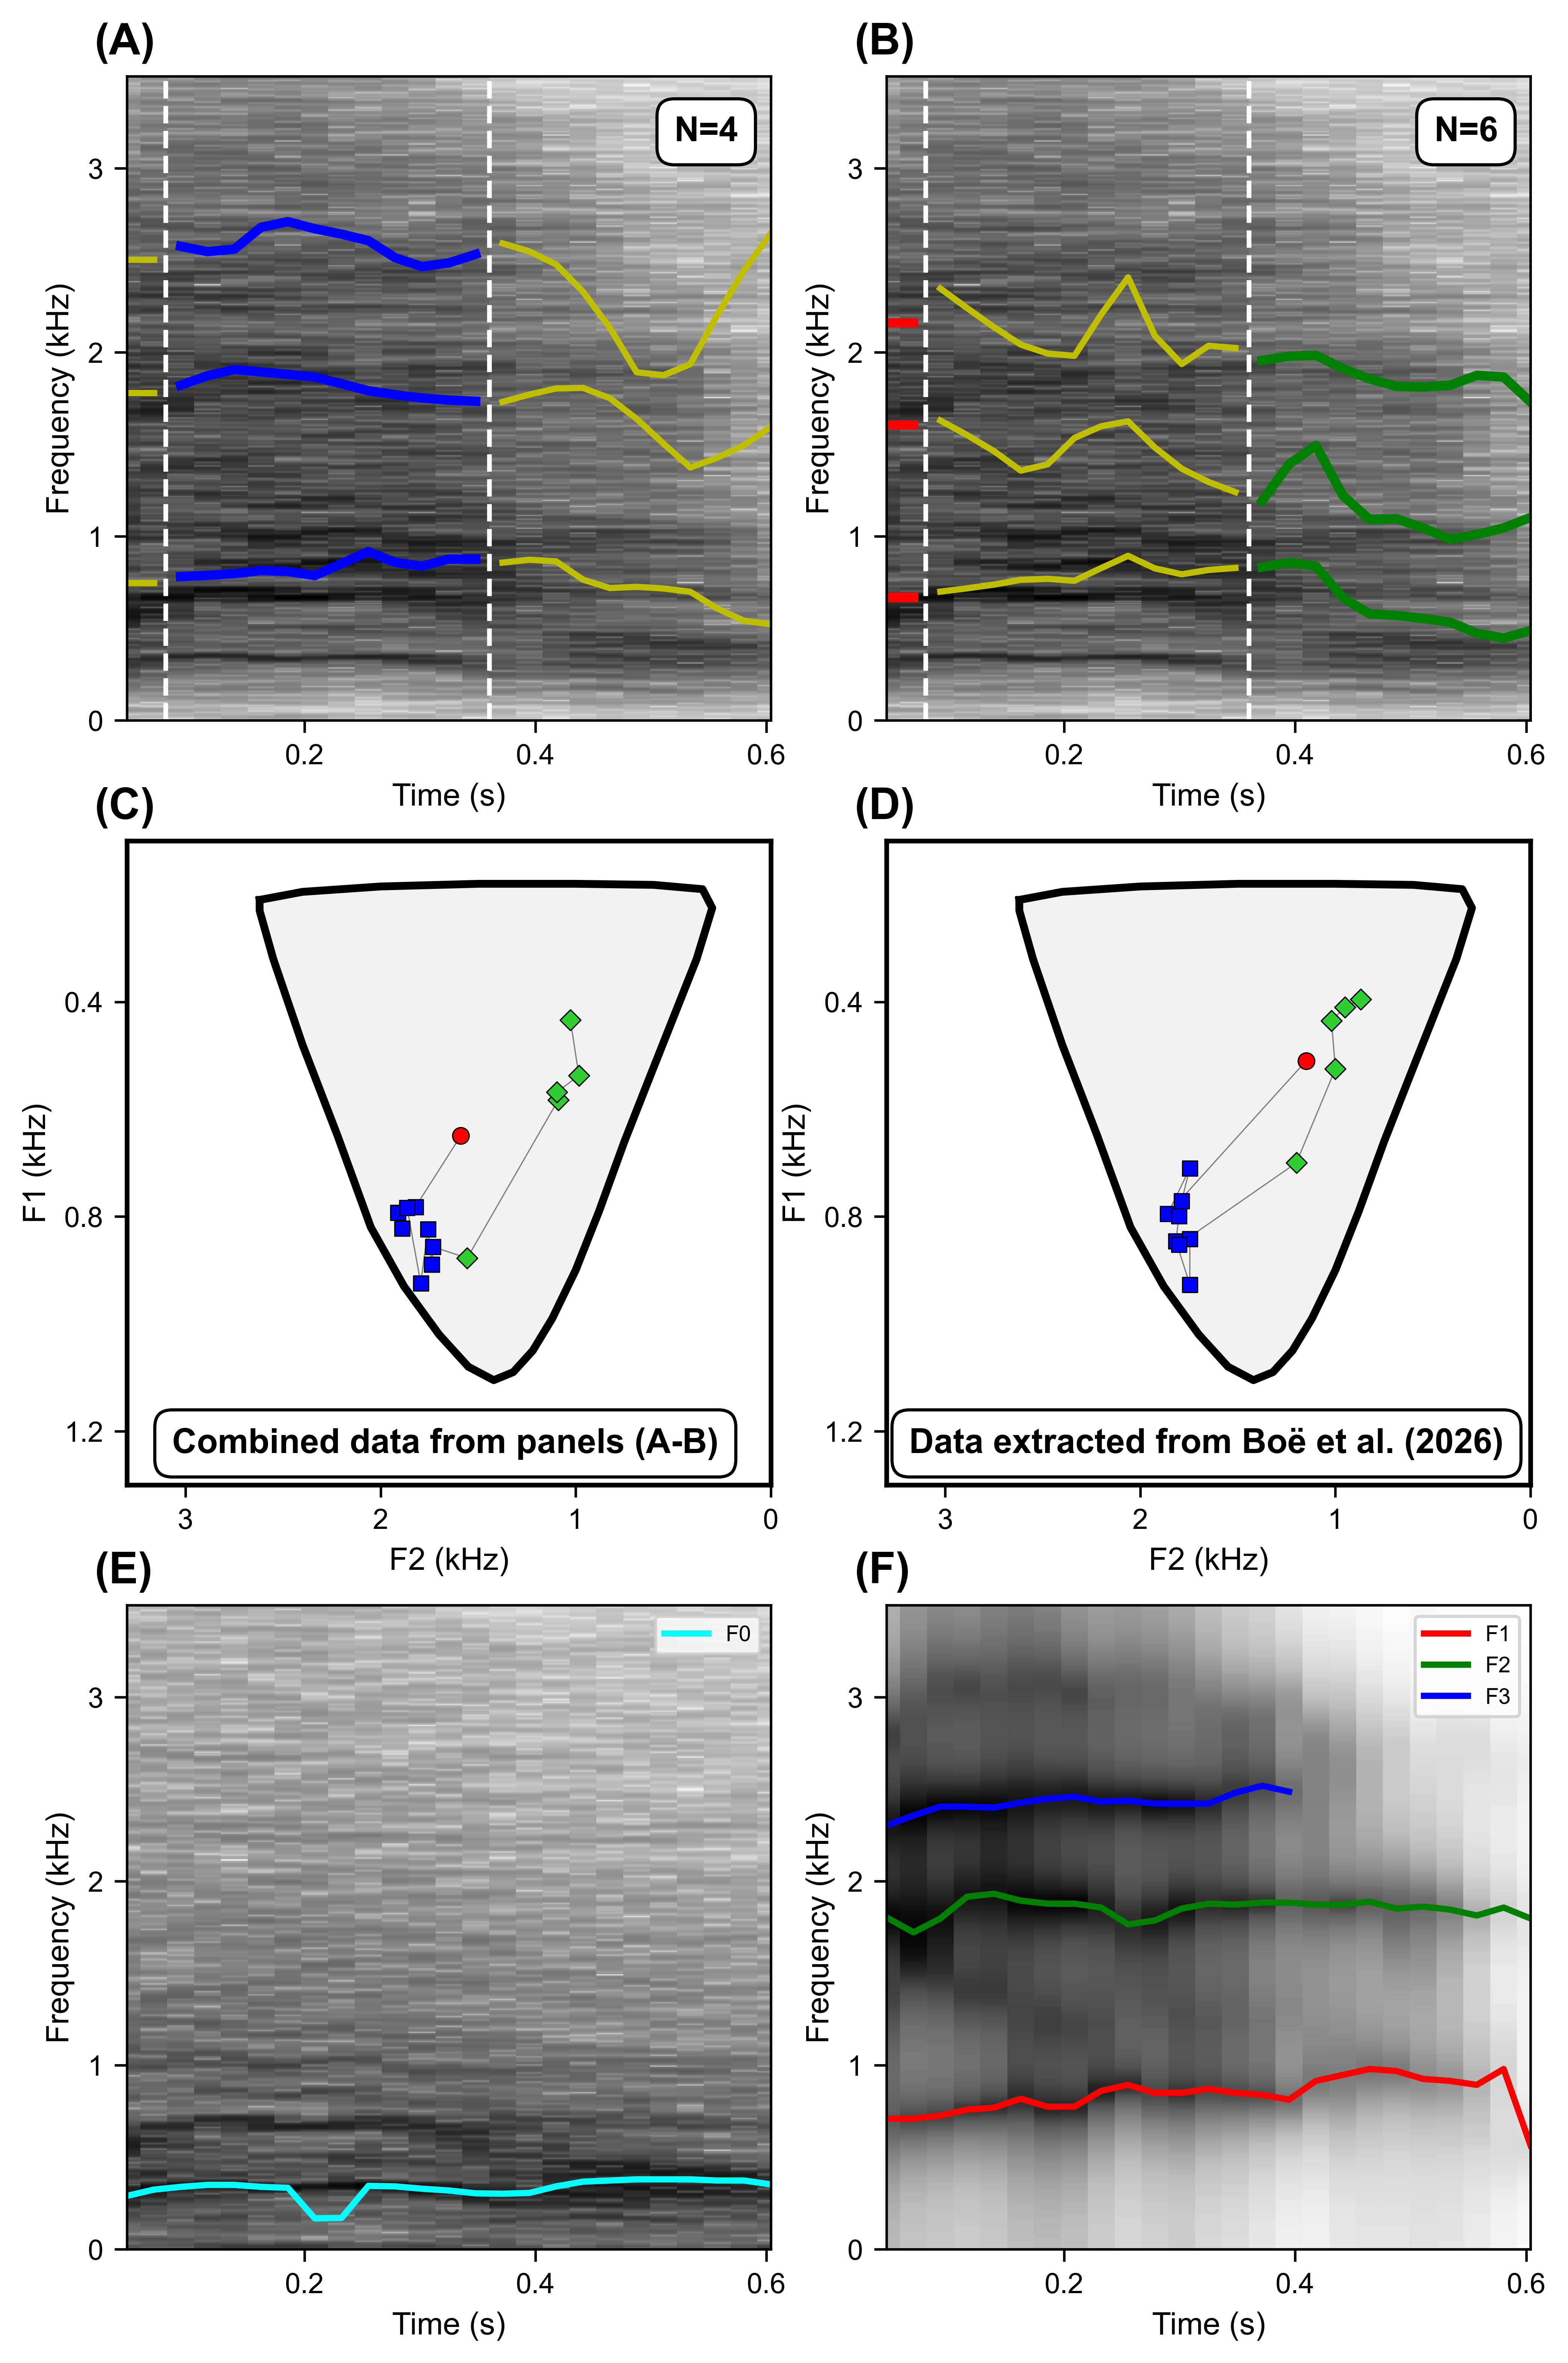
\includegraphics[width=0.8\textwidth]{../figures/analysis_3x2_panels.png}
\caption{Multi-panel analysis of a baboon wahoo call (exemplar file
\file{wahoo\_4.wav}). (A)~Wideband spectrogram of the original signal
(Hamming window, length $= 4096$ samples, hop $= 1024$ samples,
44.1\,kHz sampling rate). Overlaid formant trajectories F1--F3 (yellow
before 0.08\,s, blue between 0.08 and 0.36\,s, yellow again after
0.36\,s) were extracted using Praat's Burg algorithm via Parselmouth
(\emph{To Formant (burg)}) with parameters: time step $= 40$\,ms,
window length $= 40$\,ms, maximum formant $= 5500$\,Hz, pre-emphasis $=
50$\,Hz, number of formants $= 4$. (B)~Same as (A) but with number of
formants $= 6$; formant colours are now red for the first segment,
yellow for the middle, green for the last segment. (C)~Merged F1--F2
trajectories combining the first point from the $N=6$ extraction (red
circle) and the subsequent points from the $N=4$ extraction (blue
squares and green diamonds). The grey shaded area and black line
represent the maximal acoustic space (MAS) contour approximated from
Bo\"e et al.\ (2026). (D)~F1--F2 trajectories manually extracted from
the spectrogram published in Bo\"e et al.\ (2026) (red circle, blue
squares, green diamonds), superimposed on the same MAS contour.
(E)~Spectrogram of the glottal source estimate obtained after the second
iteration of IAIF (LPC order $= 60$). The cyan line shows the
fundamental frequency (F0) estimated from the source signal by
autocorrelation (search range 50--500\,Hz, voicing threshold $= 0.3$).
(F)~Spectrogram of the vocal-tract filter envelope $|H_{vt2}(f)|$
computed from the IAIF filter coefficients (frame-wise LPC, order $=
60$, same framing as in A and B). Overlaid formant tracks (F1 red, F2
green, F3 blue) are IAIF-based estimates obtained by peak picking on the
envelope (minimum prominence $= 2.5$\,dB, minimum peak distance $=
150$\,Hz). All spectrograms use a grey (\emph{Greys}) colour map.
Dashed white vertical lines at 0.08\,s and 0.36\,s delimit the
[w], [\textae{}] and [u] segments.}
\label{fig:multipanel}
\end{figure}

\subsection{Audio loading and resampling}

\begin{lstlisting}
def load_audio(path)
\end{lstlisting}
Loads a WAV file using \file{scipy.io.wavfile.read}, converts stereo to
mono by taking the first channel, normalises the signal to the range
$[-1, 1]$, and resamples to the target sampling frequency
$F_s = 44100$\,Hz using SciPy's \file{resample} function if necessary.
It returns the signal as a 1D numpy array and the sampling frequency.

\subsection{LPC and Levinson--Durbin recursion}

\begin{lstlisting}
def lpc_levinson(x, order)
\end{lstlisting}
Computes the linear prediction coefficients (LPC) of a given order using
the Levinson--Durbin recursion. The input \file{x} is first
mean-centred. The autocorrelation is estimated via FFT for efficiency.
The function returns the coefficient vector \file{a} (with
\file{a[0] = 1}) and the residual variance $\sigma^2$. A small
regularization is added to avoid numerical instability.

\begin{lstlisting}
def lpc_spectrum_db(a, sigma2, n_fft=4096, fs=FS_TARGET)
\end{lstlisting}
Given the LPC coefficients and the residual variance, this function
computes the frequency response of the all-pole filter
$H(f) = \sqrt{\sigma^2}\,/\,A(f)$, where $A(f)$ is the Fourier transform
of the coefficient vector. It returns the frequency axis \file{w} (in
Hz) and the magnitude spectrum in dB, computed using
\file{scipy.signal.freqz}.

\subsection{Iterative Adaptive Inverse Filtering (IAIF)}

\begin{lstlisting}
def iaif_frame(frame, fs, vt_order)
\end{lstlisting}
Performs one frame of the two-iteration IAIF algorithm to separate the
glottal source from the vocal-tract filter. The algorithm proceeds as
follows:
\begin{enumerate}
\item Estimate a first glottal filter $H_{g1}$ of order 1 via LPC, and
      inverse-filter the frame to obtain $s_1$.
\item Estimate the vocal-tract filter $H_{vt1}$ of order \file{vt\_order}
      on $s_1$.
\item Compute a first source estimate
      $g_1 = \int (H_{vt1} * \text{frame})$ and remove its mean.
\item Estimate a second glottal filter $H_{g2}$ of order 2 on $g_1$,
      inverse-filter the original frame to get $s_2$.
\item Estimate the final vocal-tract filter $H_{vt2}$ (order
      \file{vt\_order}) on $s_2$.
\item Compute the final source signal
      $g_n = \int (H_{vt2} * \text{frame})$ and remove its mean.
\end{enumerate}
The function returns $H_{vt2}$ (LPC coefficients), $\sigma^2$ (residual
variance), and the source signal $g_n$.

\subsection{Fundamental frequency estimation from the source}

\begin{lstlisting}
def estimate_f0_from_gn(gn, fs, f0_min=F0_MIN, f0_max=F0_MAX, ac_thresh=0.3)
\end{lstlisting}
Estimates the fundamental frequency F0 from a glottal source segment
\file{gn} by autocorrelation. The signal is mean-centred, then the
normalised autocorrelation is computed. The search range for the period
is derived from \file{f0\_min} and \file{f0\_max}. The peak of the
autocorrelation within this range is found; if its value exceeds
\file{ac\_thresh}, the corresponding frequency is returned; otherwise
NaN. A simple parabolic interpolation is not performed, but the index is
checked to avoid edge cases.

\subsection{Formant extraction from the LPC envelope}

\begin{lstlisting}
def get_frame_formants(frame, fs, vt_order, fmax, min_prominence, min_dist_hz)
def get_frame_formants_3(frame, fs, vt_order, fmax, min_prominence, min_dist_hz)
\end{lstlisting}
These functions extract formant frequencies from a given frame by first
performing IAIF to obtain the vocal-tract filter $H_{vt2}$, then
computing its magnitude spectrum. Peaks in the spectrum (below
\file{fmax}) are detected using \file{scipy.signal.find\_peaks} with a
minimum prominence and a minimum distance between peaks. The four most
prominent peaks (sorted by frequency) are returned as $F_1, F_2, F_3,
F_4$. The \file{get\_frame\_formants\_3} variant returns only three
formants and is used in some contexts. If fewer peaks are found, the
missing entries are filled with NaN.

\subsection{Sliding-window IAIF analysis}

\begin{lstlisting}
def iaif_sliding_analysis(x, fs)
def iaif_sliding_analysis_3(x, fs)
\end{lstlisting}
These functions apply the IAIF analysis to the entire signal using a
sliding window (Hamming window of length \file{FFT\_WIN\_LEN} and hop
size \file{HOP}). For each frame, they compute:
\begin{itemize}
\item the spectrogram of the original signal $S_{xx}$ (dB);
\item the spectrogram of the glottal source $S_{gn}$ (dB);
\item the magnitude envelope of the vocal-tract filter
      $|H_{vt2}(f)|$ (dB), interpolated onto a common frequency grid;
\item the F0 track (using \file{estimate\_f0\_from\_gn});
\item the IAIF-based formant tracks (using \file{get\_frame\_formants}).
\end{itemize}
The functions return the time axis, the frequency axis, and the four
spectral matrices, as well as the F0 track and the formant matrix. The
\file{\_3} variant returns only three formants.

\subsection{Vocal tract length estimation}

\begin{lstlisting}
def reby_mccomb_vtl_global(F1, F2, F3, F4, c=SPEED_OF_SOUND)
def reby_mccomb_vtl_global_3(F1, F2, F3, c=SPEED_OF_SOUND)
\end{lstlisting}
Computes a global vocal-tract length (VTL) estimate in cm using the
Reby--McComb formula, which fits a linear regression of formant
frequencies against odd-order numbers $(1, 3, 5, \ldots)$. The slope $b$
is obtained by $b = \sum f_i \cdot \mathrm{order} \;/\; \sum
\mathrm{order}^2$, and then $\mathrm{VTL} = c/(4b)$, where $c$ is the
speed of sound in cm/s. Only non-NaN formant values are used. Returns
NaN if fewer than two formants are available. The \file{\_3} variant
uses only three formants.

\subsection{Parselmouth formant extraction}

\begin{lstlisting}
def extract_parselmouth_formants_n(audio_path, n_form, target_times,
                                   fs_target=FS_TARGET)
\end{lstlisting}
Extracts $n$ formants from the audio file using Praat's Burg algorithm
(via Parselmouth). The function loads the sound, resamples if necessary,
and calls \emph{To Formant (burg)} with the fixed parameters (time step
$= 40$\,ms, window length $= 40$\,ms, maximum formant $= 5500$\,Hz,
pre-emphasis $= 50$\,Hz). It returns interpolated formant values $F_1,
F_2, F_3$ at the specified \file{target\_times} (time axis from the IAIF
analysis), as well as the raw formant tracks at Parselmouth's own time
grid. The interpolation handles missing values by using only valid
frames.

\subsection{Visualisation utilities}

\begin{lstlisting}
def plot_f1f2_trajectory(ax, F1, F2, marker_type, marker_color, xlim, ylim)
\end{lstlisting}
Draws an F2--F1 trajectory on a given Matplotlib axis. It overlays the
maximal acoustic space (MAS) contour (grey shaded area and black
outline) defined by the hardcoded arrays \file{MAS\_F1\_closed} and
\file{MAS\_F2\_closed}. The trajectory is plotted as a thin grey line,
and each point is marked according to the provided \file{marker\_type}
and \file{marker\_color}. The axis limits, labels, and tick settings are
also configured.

\begin{lstlisting}
def setup_frequency_axis(ax)
def add_panel_label(ax, label)
def fix_initial_nan(arr)
\end{lstlisting}
\file{setup\_frequency\_axis} sets the common style for spectrogram
axes: limits (0--3.5\,kHz), ticks every 1\,kHz on the y-axis and 0.2\,s
on the x-axis, and labels. \file{add\_panel\_label} adds a bold panel
label (e.g., ``(A)'') in the top-left corner of an axis.
\file{fix\_initial\_nan} replaces a NaN first element of an array by the
first non-NaN value, to avoid gaps at the beginning of formant tracks
when plotting.

\subsection{Main figure assembly}

\begin{lstlisting}
def make_figure(x, fs, audio_path, out_path)
\end{lstlisting}
This is the master function that orchestrates the entire analysis and
creates the $3\times2$ panel figure (Fig.~\ref{fig:multipanel}). It
performs the following steps:
\begin{enumerate}
\item Runs \file{iaif\_sliding\_analysis} to obtain all IAIF-derived
      data.
\item Computes VTL from the IAIF formants.
\item Extracts Parselmouth formants for $N=4$ and $N=6$ using
      \file{extract\_parselmouth\_formants\_n}.
\item Builds a 3-row, 2-column grid with
      \file{matplotlib.gridspec.GridSpec}.
\item Plots panels (A) through (F) as described in the caption of
      Fig.~\ref{fig:multipanel}.
\item Adds panel labels, dashed vertical lines at 0.08 and 0.36 seconds,
      and a consistent colour map.
\item Saves the figure at 600 dpi.
\end{enumerate}

\subsection{Single-pulse extraction}

\begin{lstlisting}
def extract_and_save_glottal_pulse(x, fs, png_path)
\end{lstlisting}
This function extracts a single glottal pulse from a stable portion of
the signal (between 0.26 and 0.34\,s). It applies IAIF on a
Hamming-windowed segment to obtain the source $g_n$, then estimates the
fundamental period via autocorrelation. A single pulse is isolated
around the maximum of the absolute source signal, and a time-domain plot
is saved as a PNG file (\file{glottal\_pulse.png}, reproduced here as
Fig.~\ref{fig:pulse}). This function is called separately in the main
block.

\begin{figure}[t]
\centering
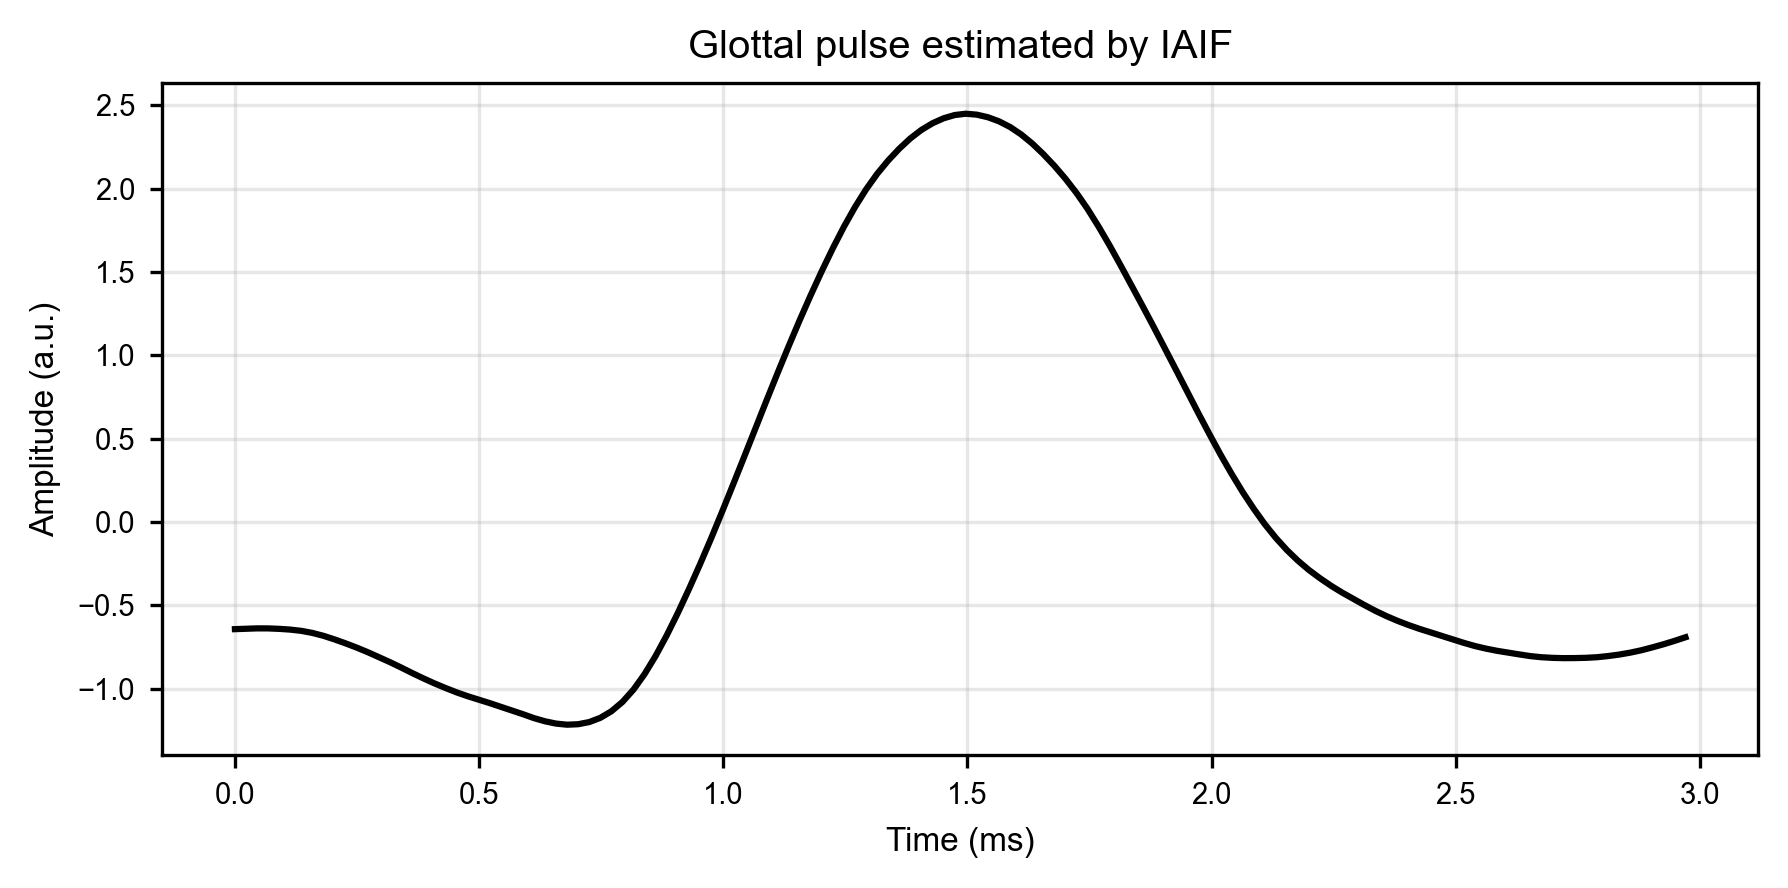
\includegraphics[width=0.6\textwidth]{../figures/glottal_pulse.png}
\caption{Single glottal pulse estimated by IAIF on the segment
260--340\,ms of \file{wahoo\_4.wav} (Hamming window, autocorrelation
period, extraction around the largest absolute excursion of the source
signal).}
\label{fig:pulse}
\end{figure}

\subsection{Main execution block}

The script, when run as a standalone program, reads an audio file either
from the command line or uses a default filename (\file{wahoo\_4.wav}).
It then loads the audio, calls
\file{extract\_and\_save\_glottal\_pulse}, and calls \file{make\_figure}
to produce the multi-panel figure shown in this supplement
(Fig.~\ref{fig:multipanel}).

The script is designed to be fully reproducible; all parameters are
hardcoded as constants, and the code is provided verbatim in the
repository (\file{supplementary/original\_scripts/}). All functions are
self-contained and rely only on the imported libraries, ensuring that
the entire analysis can be replicated on any system with Python and the
required packages installed.

%======================================================================
\section{F0 contour with filtered autocorrelation (\file{make\_figure\_ac.py})}

\begin{figure}[t]
\centering
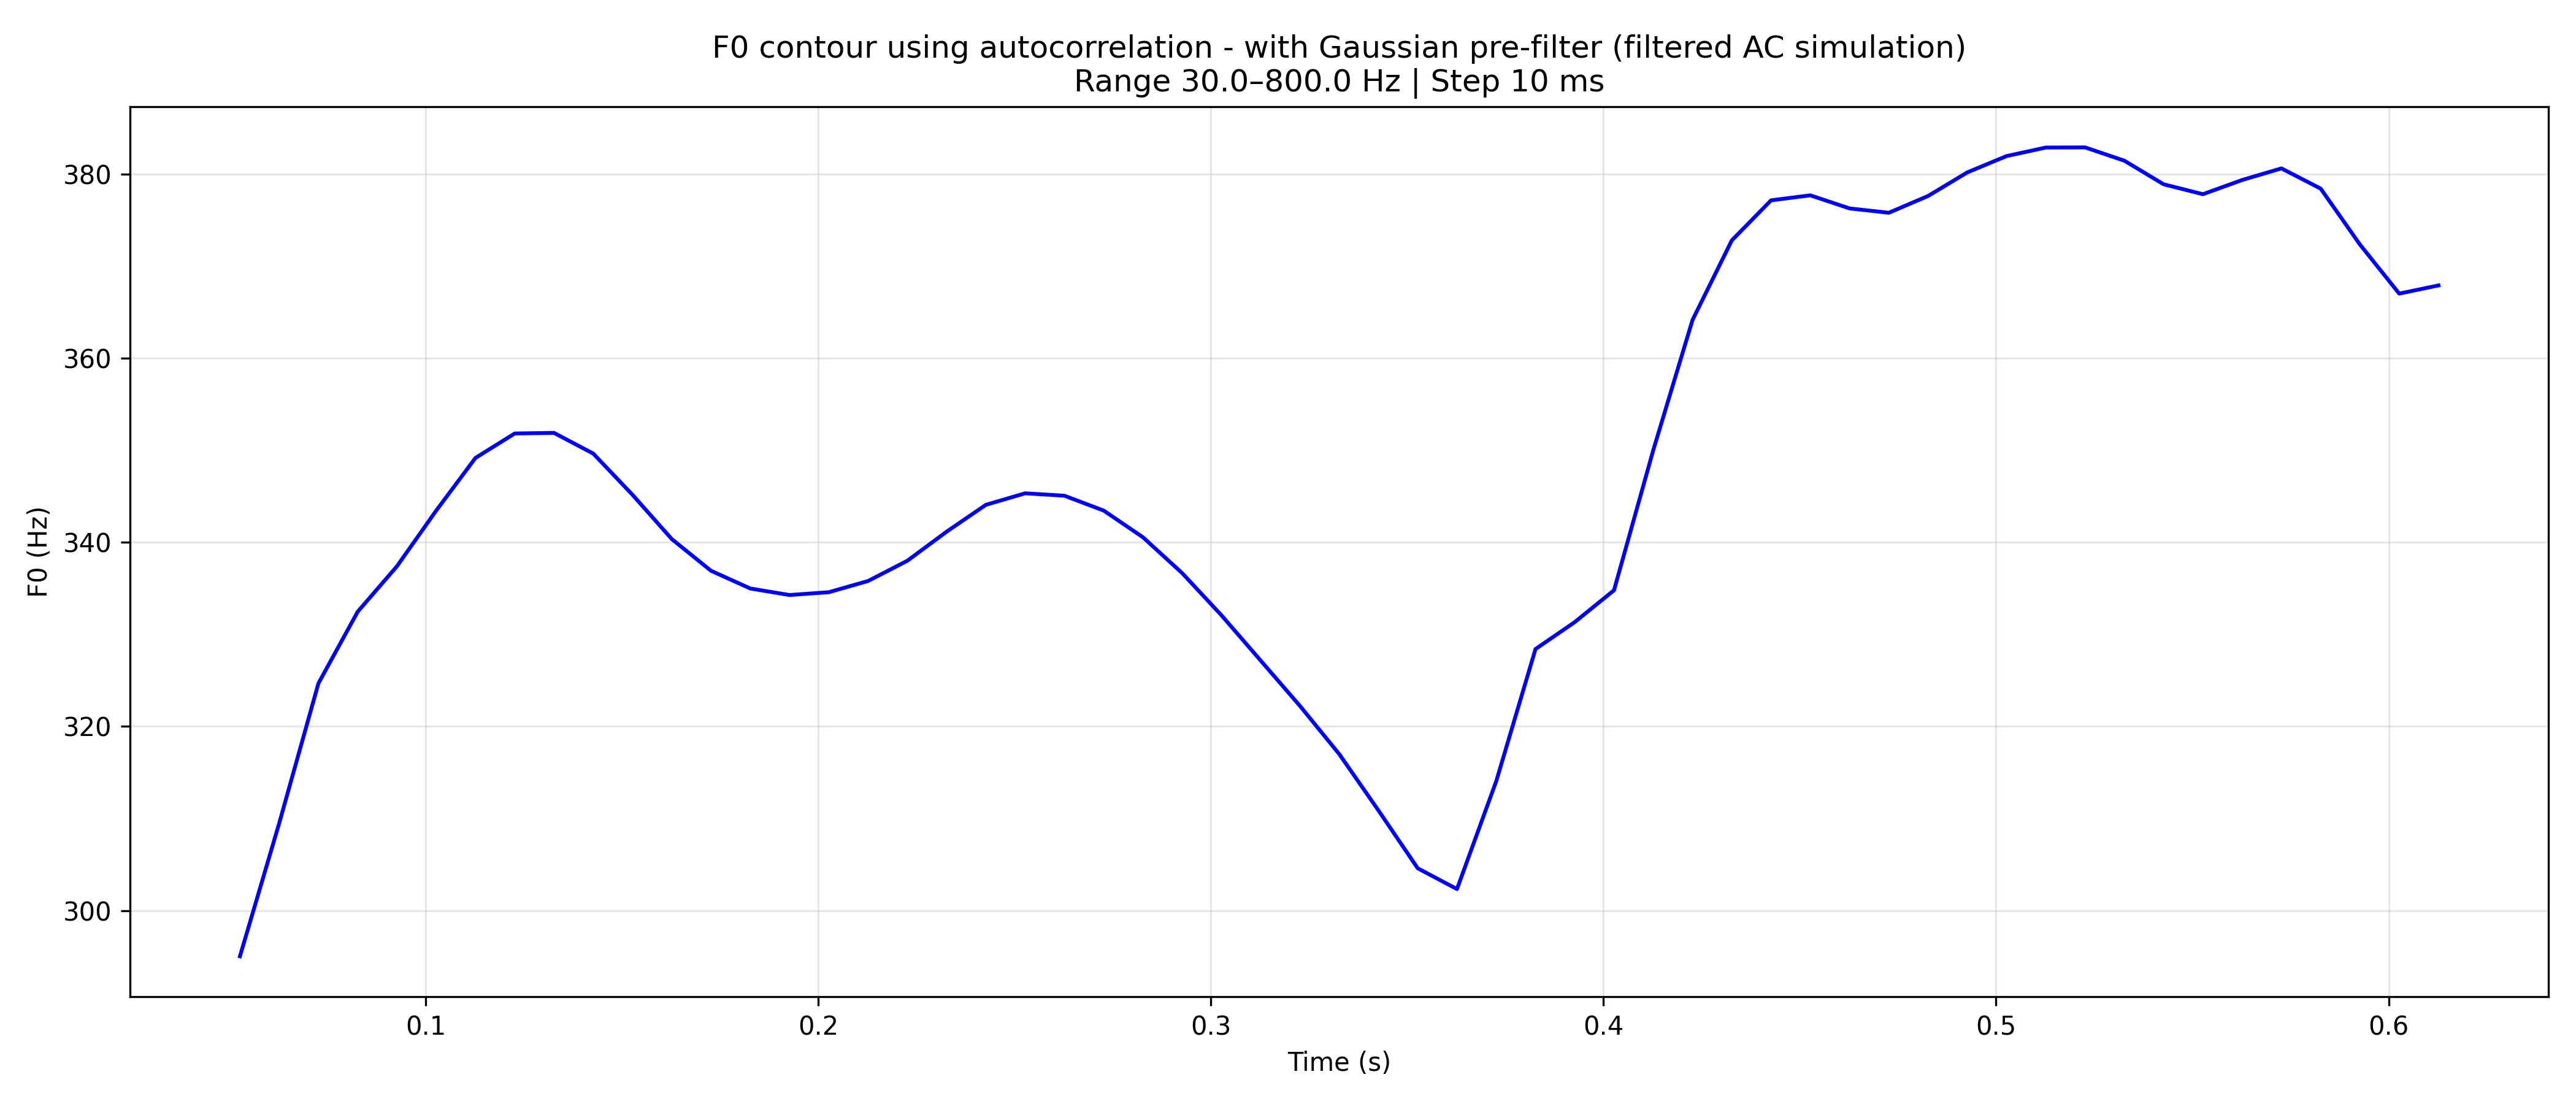
\includegraphics[width=0.95\textwidth]{../figures/wahoo_4_f0_filtered_ac.png}
\caption{F0 contour obtained after Gaussian low-pass pre-filtering
(cutoff 800\,Hz, attenuation $-30.5$\,dB at cutoff) followed by Praat's
autocorrelation pitch algorithm (\emph{to\_pitch\_ac}) with floor
30\,Hz, ceiling 800\,Hz, and time step 0.01\,s. The analysis yielded 57
voiced frames, a mean F0 of 348.2\,Hz (standard deviation 24.3\,Hz).
This preprocessing effectively suppresses subharmonics and produces a
smooth pitch track comparable to Praat 6.4.65's \emph{To Pitch (filtered
ac)\ldots} command.}
\label{fig:f0}
\end{figure}

\begin{figure}[t]
\centering
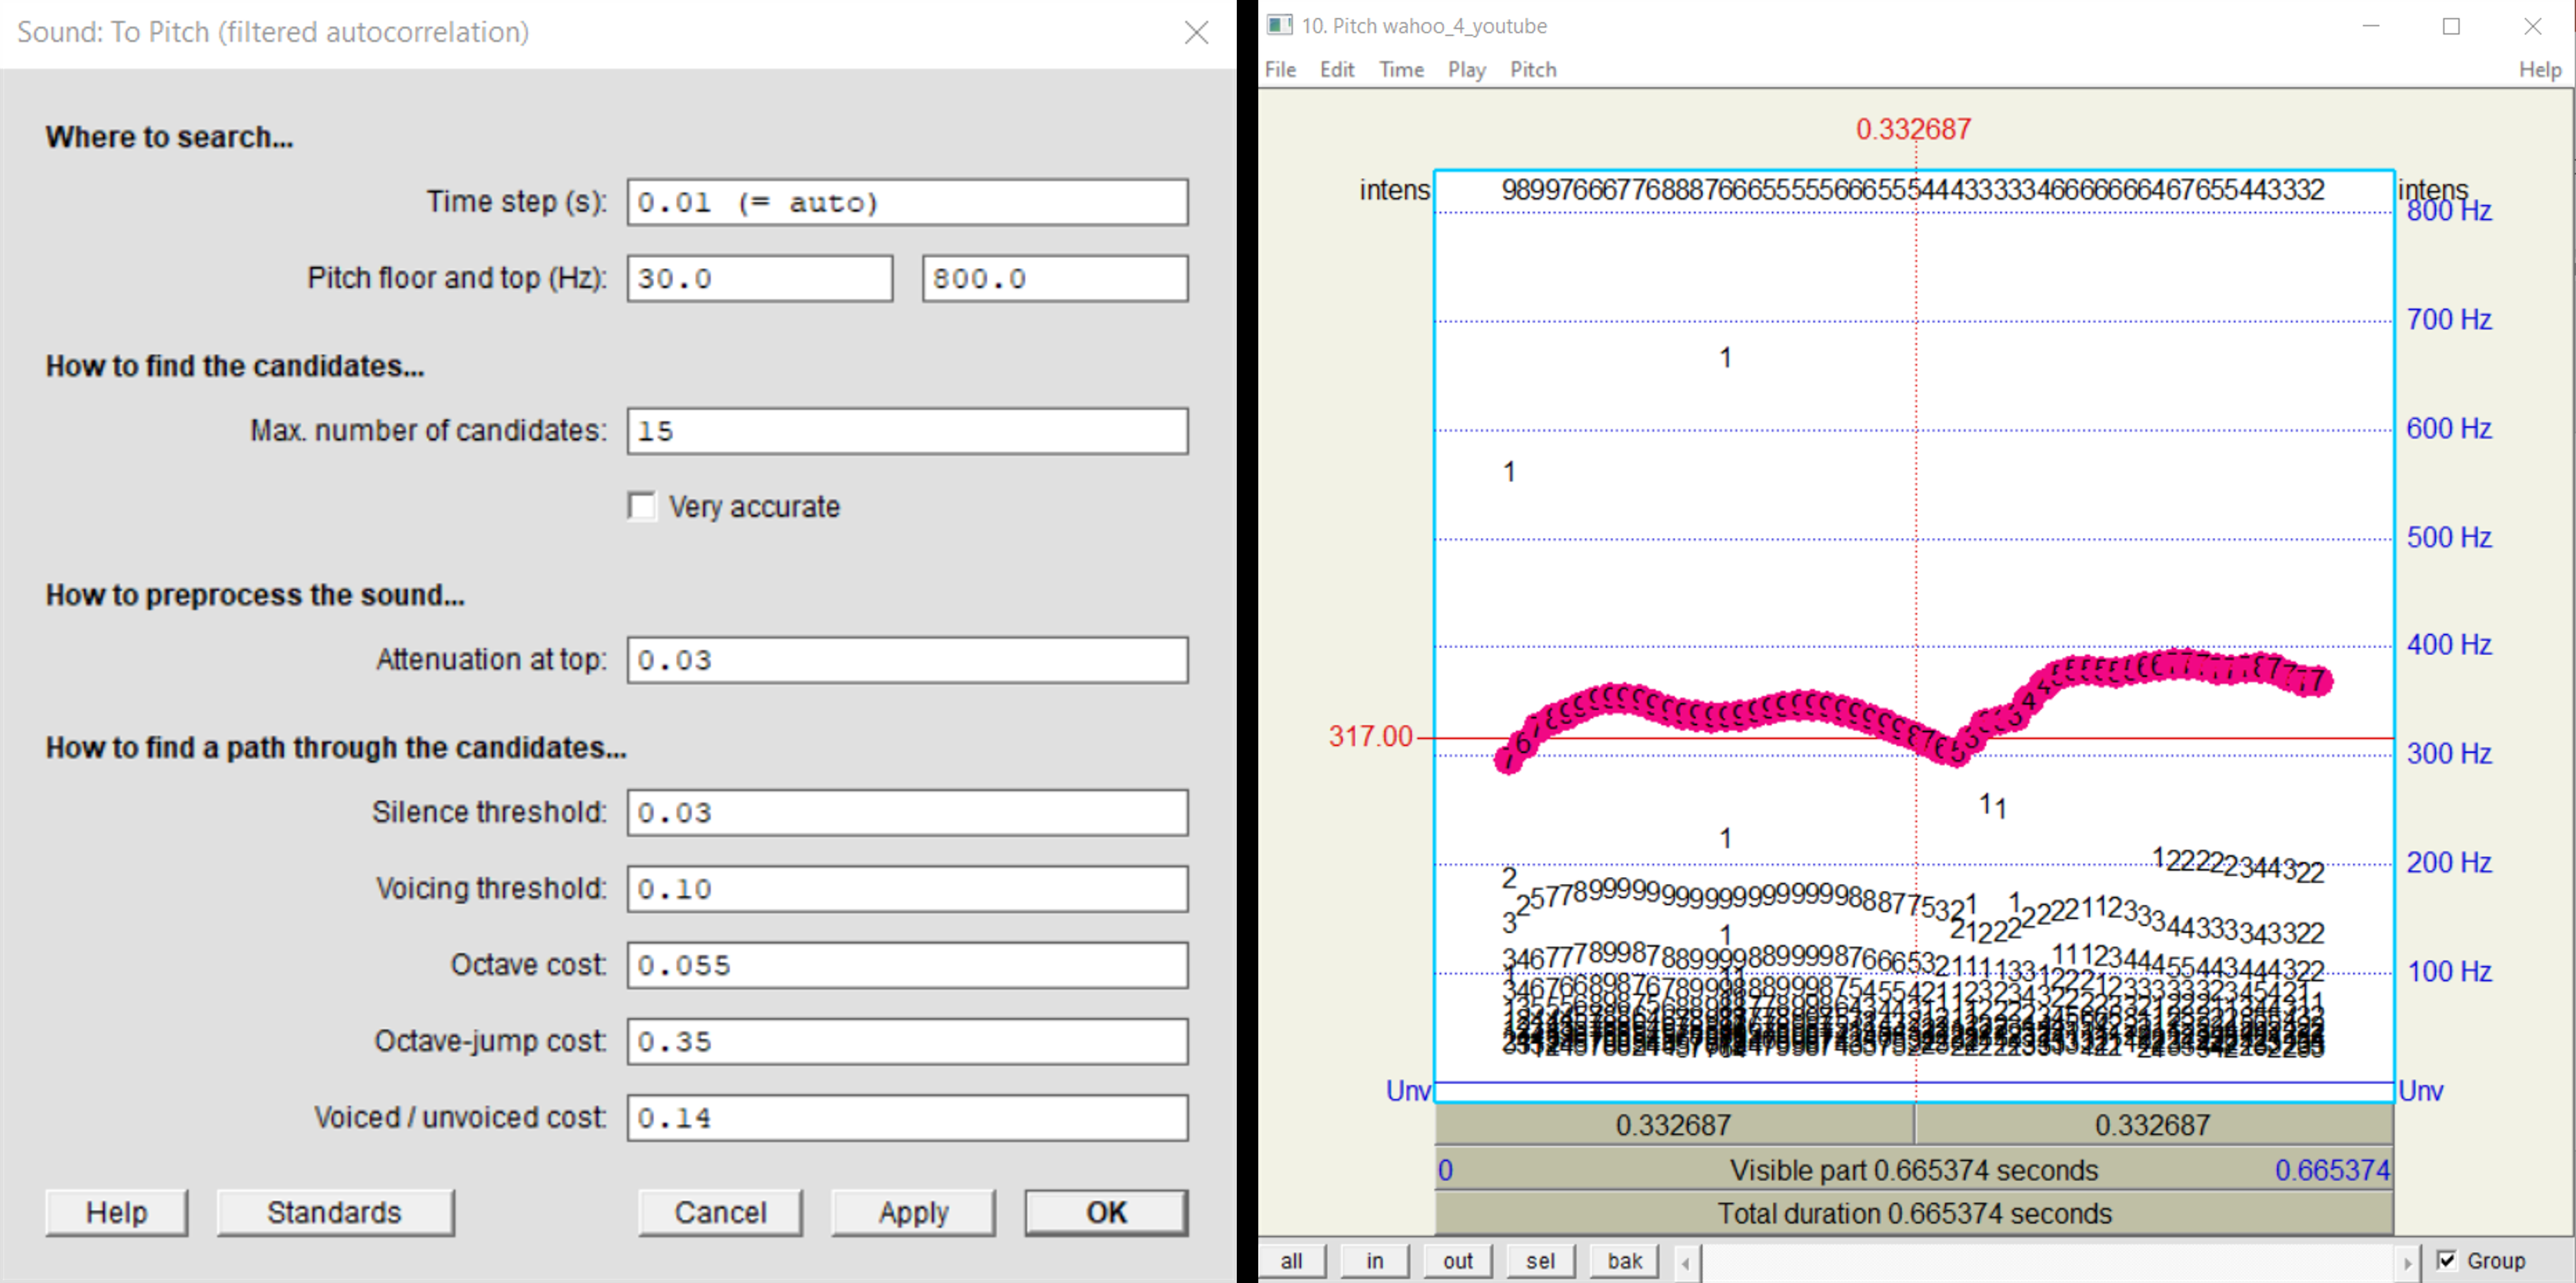
\includegraphics[width=0.95\textwidth]{../figures/praat_filtered_ac_settings.png}
\caption{Left: settings of Praat 6.4.65's \emph{To Pitch (filtered
autocorrelation)} command. Right: resulting pitch contour of
\file{wahoo\_4.wav} displayed in Praat (mean 317\,Hz over the visible
part). The Python pre-filtering of \file{make\_figure\_ac.py} replicates
this behaviour.}
\label{fig:praat}
\end{figure}

Figure~\ref{fig:f0} is produced with the Python program
\file{make\_figure\_ac.py}. To replicate the behavior of the
\emph{filtered autocorrelation} method available in Praat 6.4.65 (but
not in the legacy Praat version embedded in Parselmouth 0.4.5), a
Gaussian low-pass filter is applied to the time-domain signal prior to
pitch extraction. This preprocessing step attenuates high-frequency
components above a cutoff frequency $f_{\mathrm{cutoff}}$ with a smooth
roll-off, effectively removing spectral energy that could otherwise
produce subharmonic false peaks in the autocorrelation function.

Subharmonics --- often arising from irregular vocal fold vibration or
background noise --- manifest as additional periodicities at integer
fractions of the true fundamental period. By suppressing frequencies
above $f_{\mathrm{cutoff}}$ (set here to 800\,Hz, which is also used as
the pitch ceiling in Praat's filtered autocorrelation), the filter
preserves the dominant periodicity while reducing the amplitude of
spurious subharmonic candidates.

The filter is implemented in the frequency domain using a fast Fourier
transform (FFT), applying a Gaussian window
$H(f) = \exp\!\left(-(f/\sigma)^2/2\right)$ with
$\sigma = f_{\mathrm{cutoff}} / \sqrt{-2\ln(\alpha)}$, where $\alpha$ is
the desired attenuation at $f_{\mathrm{cutoff}}$ (here $\alpha = 0.03$,
corresponding to $-30.5$\,dB). The filtered signal is then transformed
back to the time domain via inverse FFT.

This preprocessing step, combined with the standard autocorrelation
pitch algorithm (Praat's \file{to\_pitch\_ac}) using a pitch floor of
30\,Hz, a pitch ceiling of 800\,Hz, and a time step of 0.01\,s, yields a
fundamental frequency contour that closely matches that obtained from
Praat 6.4.65's \emph{To Pitch (filtered ac)\ldots} command
(Fig.~\ref{fig:praat}), effectively mitigating octave-halving errors and
improving robustness in the presence of subharmonics.

%======================================================================
\section{Analysing the glottal pulse extracted with IAIF\\ (\file{make\_figure\_glottal.py})}

This Python script performs a comprehensive analysis of the glottal
source waveform extracted from a voiced signal. It uses Iterative
Adaptive Inverse Filtering (IAIF) to separate the glottal flow
derivative from the vocal-tract filter, then produces a four-panel
figure showing the pulse train, phase portrait, spectrogram, and
long-term average spectrum (Figs.~\ref{fig:wa} and \ref{fig:hoo}). The
script is designed to run from the command line and requires NumPy,
SciPy, Matplotlib, and optionally Parselmouth for resampling.

\subsection{Core signal processing functions}

\file{lpc\_levinson(x, order)} computes linear prediction coefficients
(LPC) using the Levinson--Durbin recursion. Returns the coefficient
vector \file{a} (with \file{a[0] = 1}) and the residual variance
$\sigma^2$. The autocorrelation is estimated via FFT for efficiency.

\file{iaif\_frame(frame, fs, vt\_order)} performs the two-iteration IAIF
algorithm on a single frame. It returns the vocal-tract filter
coefficients $H_{vt2}$, the residual variance, and the glottal source
signal $g_n$. The algorithm is described in detail in
Section~1 of this supplement.

\file{estimate\_f0\_from\_gn(gn, fs, f0\_min, f0\_max, ac\_thresh)}
estimates the fundamental frequency from the glottal source segment
\file{gn} using autocorrelation. The search range is determined by
\file{f0\_min} and \file{f0\_max}; the peak of the normalised
autocorrelation must exceed \file{ac\_thresh} (default 0.3) to be
accepted. Returns the estimated F0 in Hz, or NaN if no reliable peak is
found.

\file{normalize\_amplitude(signal, fs, cutoff, order, eps)} centres and
normalises the amplitude of a glottal signal. It removes slow drifts
(floating DC) by subtracting a low-pass filtered version, and divides by
a low-pass filtered envelope to flatten the overall amplitude. This
preprocessing is essential for phase portrait visualisation because it
removes amplitude modulation that could obscure the underlying dynamics.

\file{plot\_phase\_portrait(signal, fs, title, ax, color, alpha, lw,
normalize)} generates a phase portrait in the Hilbert plane. It computes
the analytic signal via the Hilbert transform, normalises the real and
imaginary parts, and plots the trajectory. If \file{normalize} is True,
the amplitude normalisation is applied first. The function returns the
Matplotlib axis object.

\file{extract\_full\_glottal\_train(x, fs, vt\_order, win\_len, hop)}
reconstructs the full glottal source waveform from the input signal
\file{x} using overlap-add (OLA). The signal is divided into
Hann-windowed frames, IAIF is applied to each frame, and the resulting
source segments are summed with appropriate window normalisation.
Returns the time axis and the reconstructed glottal signal.

\file{load\_audio(path, target\_fs)} loads a WAV file, converts to mono,
normalises to $[-1, 1]$, and resamples to the target sampling rate (if
necessary). Uses Parselmouth if available, otherwise falls back to
\file{scipy.signal.resample\_poly}.

\subsection{Execution and command-line usage}

The script is executed as:
\begin{lstlisting}[language=bash]
python make_figure_glottal.py [audio_file.wav]
\end{lstlisting}
If no argument is provided, it defaults to \file{wahoo\_4.wav}. The
``wa'' (100--260\,ms) and ``hoo'' (390--550\,ms) analysis segments are
selected by the \file{WA} constant at the top of the file, and the
output figure is saved as
\file{glottal\_train\_analysis\_wa.png} or
\file{glottal\_train\_analysis\_hoo.png} accordingly.

\subsection{Dependencies}

The script requires NumPy, SciPy, and Matplotlib. For automatic
resampling, Parselmouth is recommended but not mandatory. All other
functions are self-contained. The code is fully reproducible and the
parameters can be adjusted at the top of the file to suit different
signals or analysis needs.

\begin{figure}[p]
\centering
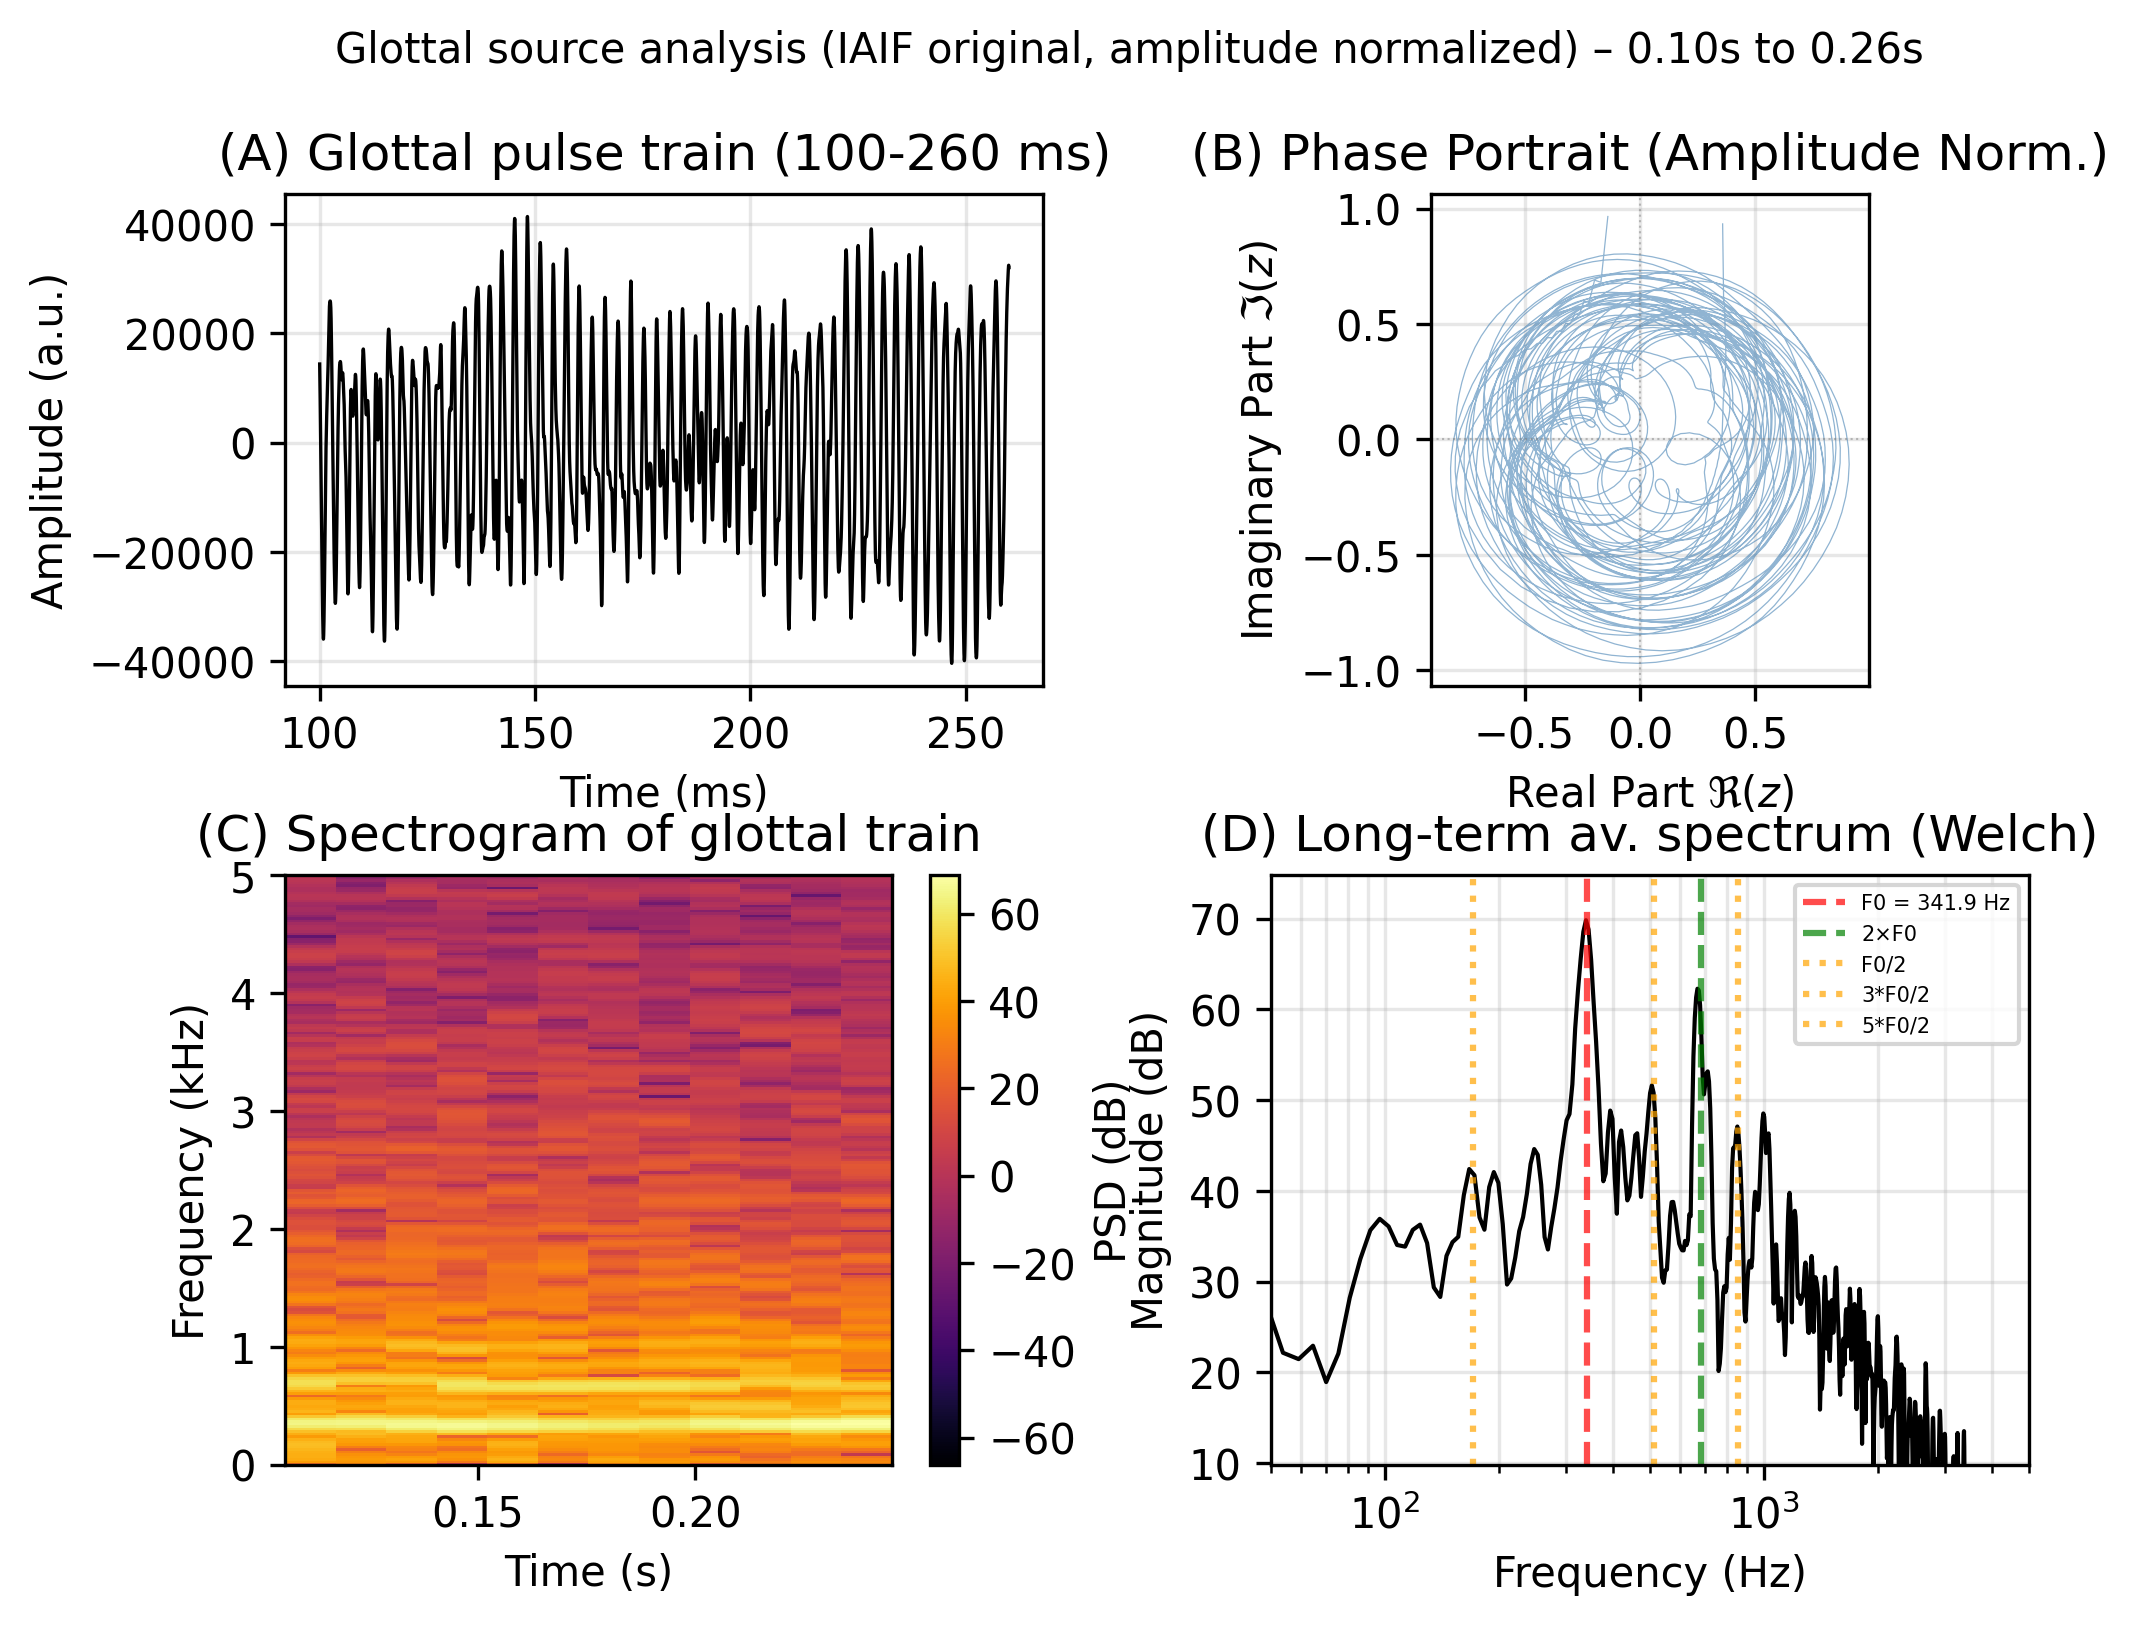
\includegraphics[width=0.62\textwidth]{../figures/glottal_train_analysis_wa.png}
\caption{Glottal source analysis (IAIF) --- ``wa'' segment
(100--260\,ms). (A)~Glottal pulse train: the amplitude does not
systematically alternate between successive cycles, preventing a
definitive conclusion of period doubling. (B)~Phase portrait (Hilbert
plane): the trajectory forms a thickened annular band rather than a
single closed loop. (C)~Spectrogram: while a fundamental harmonic and
possibly some sub-harmonics are present in the source, the two-frequency
dynamics is not visibly apparent. (D)~Long-term average spectrum
(Welch): in addition to the dominant peak at $F_0 = 341.9$\,Hz, spectral
ridges appear at $F_0/2$, $3F_0/2$, and $5F_0/2$ (orange dotted lines),
though their energy is substantially lower than that of the integer
harmonics. \emph{Conclusion:} taken together, these features indicate
that the glottal source deviates from a purely harmonic and decreasing
(e.g., $-12$\,dB/octave) spectral model, challenging the linear
source--filter separation assumption for this segment.}
\label{fig:wa}
\end{figure}

\begin{figure}[p]
\centering
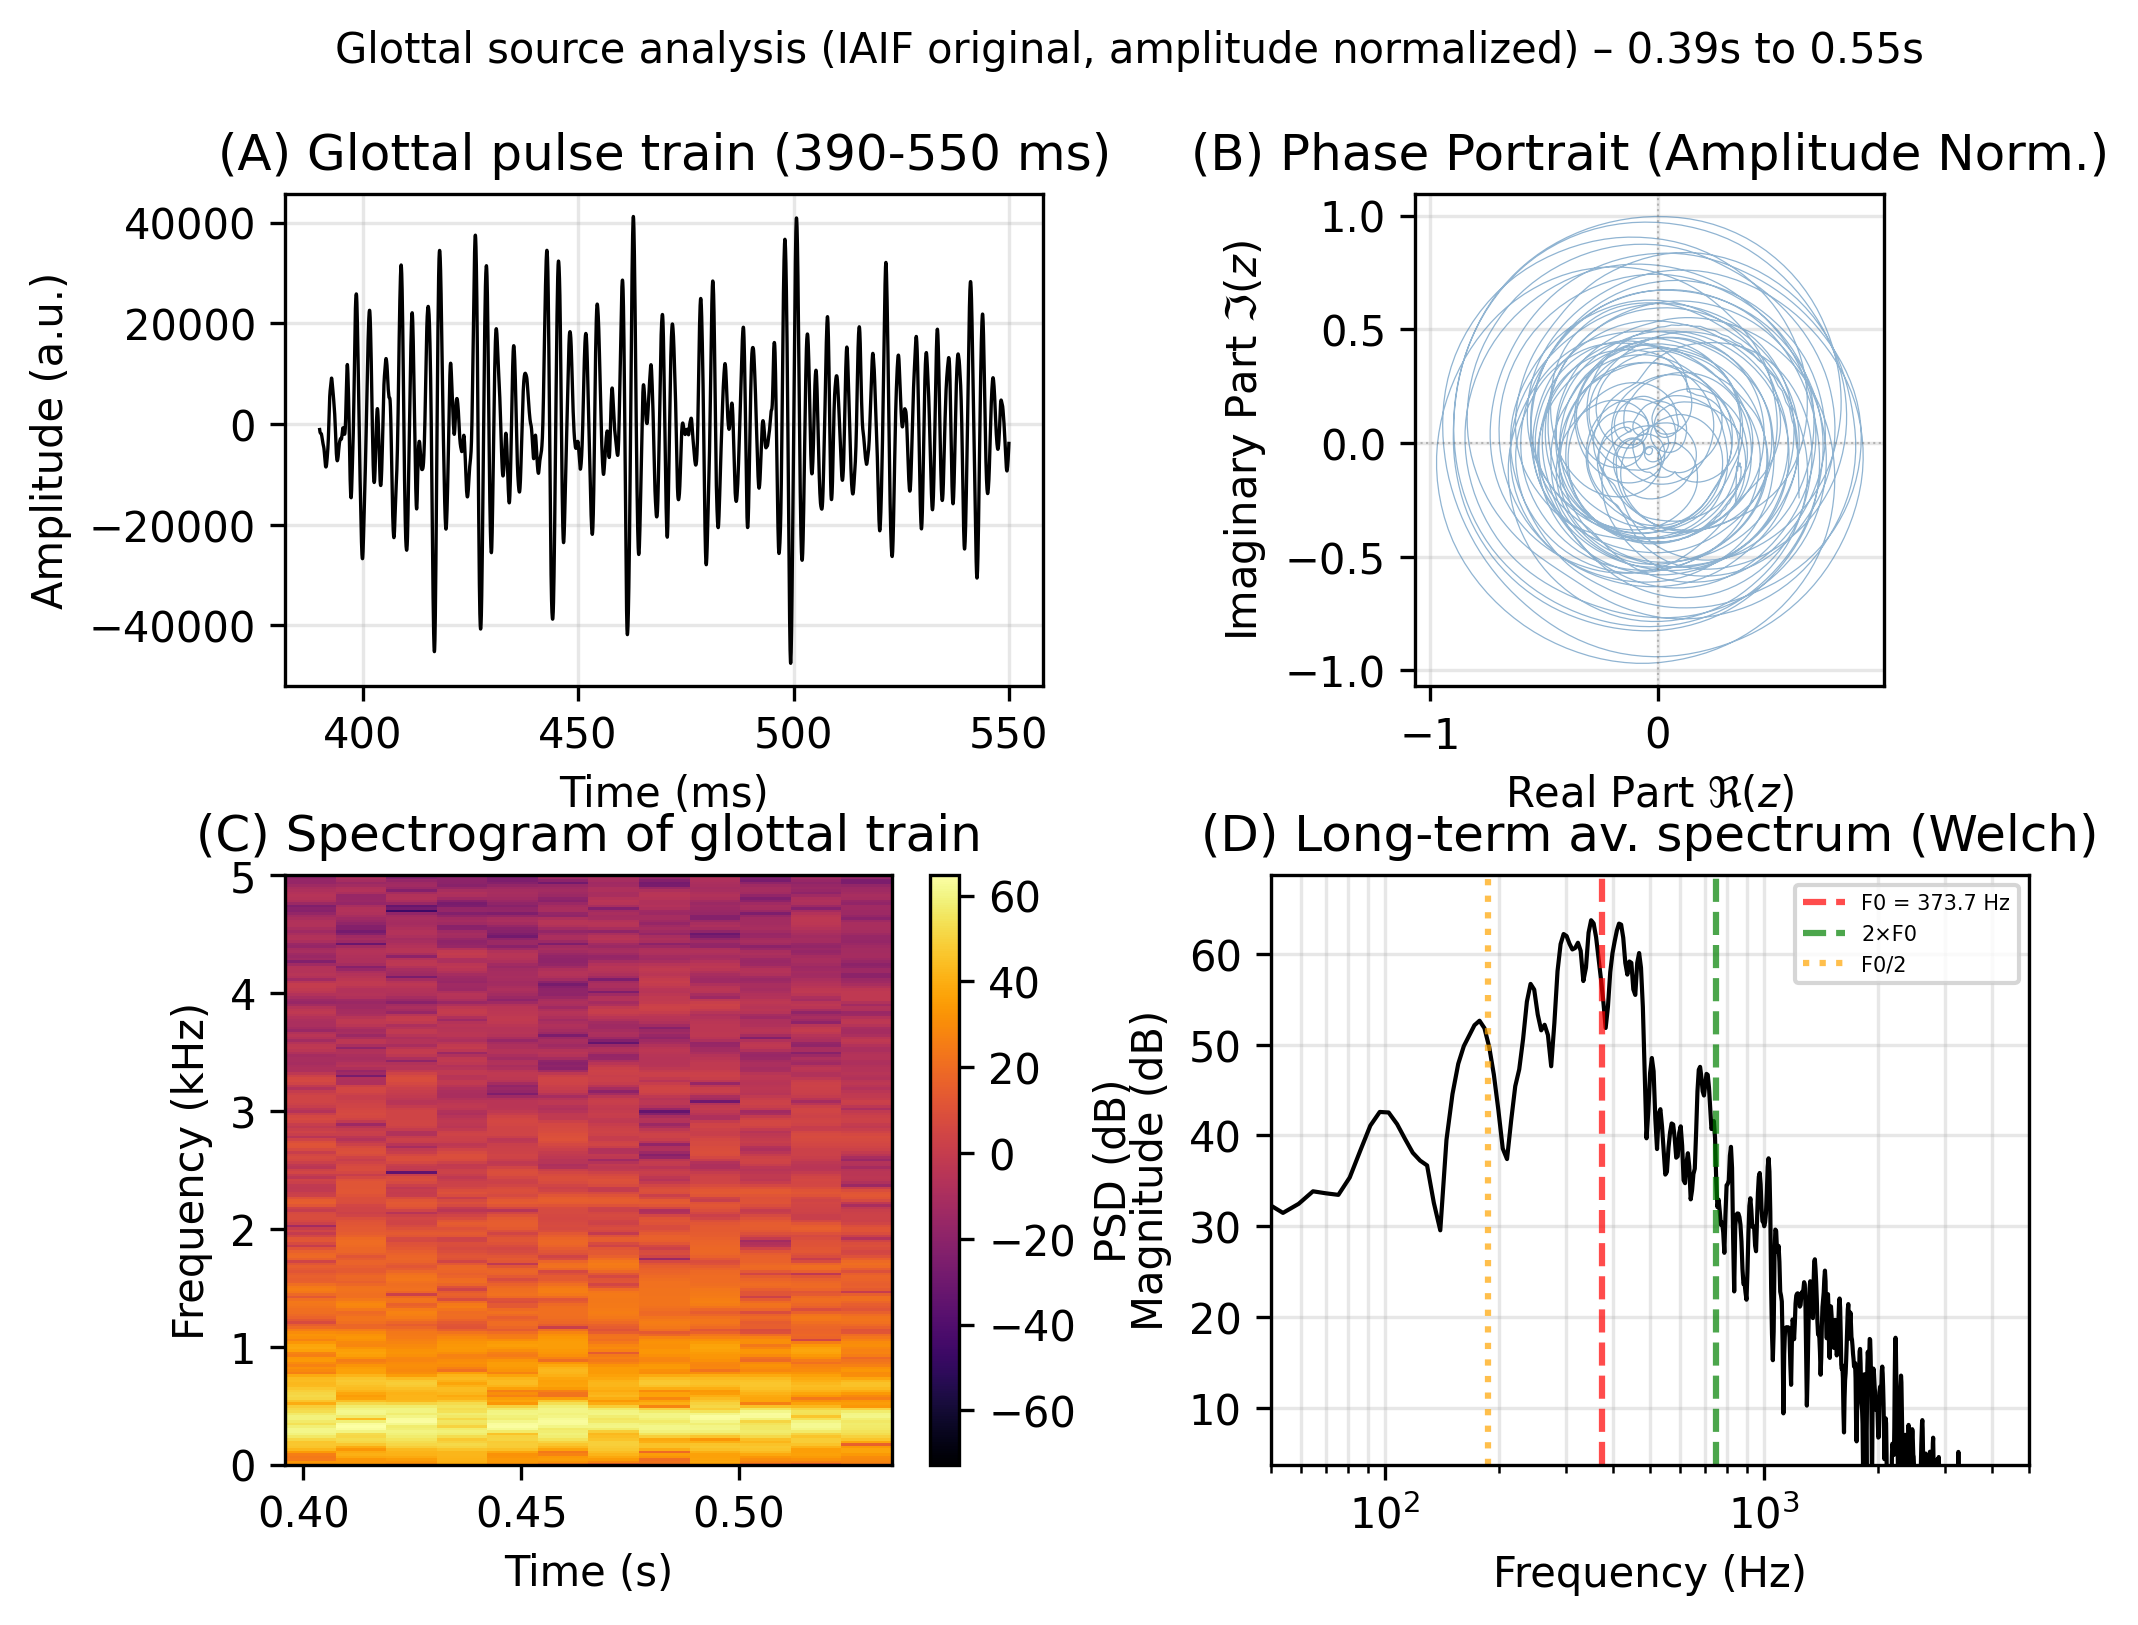
\includegraphics[width=0.62\textwidth]{../figures/glottal_train_analysis_hoo.png}
\caption{Glottal source analysis (IAIF) --- ``hoo'' segment
(390--550\,ms). (A)~Glottal pulse train: cycle-to-cycle amplitude and
timing are strongly irregular with no discernible repeating pattern,
indicating a breakdown of any low-period orbital structure present in
the earlier segment. (B)~Phase portrait (Hilbert plane): the trajectory
fills a broad, irregular disk extending beyond unit radius, with no
coherent winding structure; this irregular geometry evokes a
chaotic-like dynamical regime, although a more precise characterization
would require additional analysis. (C)~Spectrogram: a broad and thick
spectral peak is observed, with a weak harmonic structure, superimposed
on a continuous noise floor. (D)~Long-term average spectrum (Welch): the
fundamental peak is substantially broadened, while a prominent
subharmonic peak appears near $F_0/2$ and weak harmonic peaks near
$2F_0$; a continuous spectral background is visible between harmonic
ridges. \emph{Conclusion:} taken together, these observations indicate a
marked departure from a regular periodic source, where the aperiodicity
is sufficiently severe to challenge the linear source--filter
separation, and therefore any LPC-based formant estimate, for this
segment.}
\label{fig:hoo}
\end{figure}

%======================================================================
\section{Re-analysis of the published formant trajectories\\ (\file{make\_figure\_1.py})}

Figure~1 of the article is produced by \file{make\_figure\_1.py}. The
script extracts Praat/Burg formant tracks of \file{wahoo\_4.wav} with
$N=4$ and $N=6$ LPC poles, builds the merged trajectory using the
optimal $N$ per segment (first frame from $N=6$, frames 2--9 from $N=4$,
remaining frames from $N=6$), reads the reference tracks digitized from
Bo\"e et al.\ (2026, their Fig.~10h), and computes one Reby--McComb VTL
estimate per panel. The three panels are drawn with the same
comparison-panel style as the article (grey dashed reference with open
markers; black estimated tracks with colour-coded initial/medial/final
markers) and a shared legend. Running
\file{python make\_figure\_1.py} reproduces the article figure and
prints the four VTL estimates.

%======================================================================
\section{Repository contents}

The complete material is archived in the \file{baboon-acoustics}
repository, of which this supplement is part:
\begin{itemize}
\item \file{baboon\_acoustics/} --- refactored, documented Python
      package implementing the same algorithms (formants Praat/Burg and
      IAIF, F0, VTL, glottal source, plotting);
\item \file{supplementary/original\_scripts/} --- the four original
      scripts described in this document, archived verbatim;
\item \file{supplementary/figures/} --- all figures of the article and
      of the present supplement;
\item \file{data/} --- the audio material: the four wahoo calls of the
      sequence (\file{wahoo\_1.wav} \ldots{} \file{wahoo\_4.wav}), the
      full original recording (\file{The\_Baboon\_Bark.wav}), and the
      reference F0 table (\file{wahoo\_4\_f0\_filtered\_ac.csv});
\item \file{examples/, scripts/, demos/, tests/, docs/} --- guided
      example, figure-reproduction scripts, interactive HTML demos, unit
      tests and the user documentation of the package.
\end{itemize}

\section*{Reference}
\small
Bo\"e, L.-J., Laporte, M., Sawallis, T.\,R., Badin, P., \& Schwartz,
J.-L. (2026). Stalking the wild formant: How to reliably measure
formants in primate vocalizations. \emph{International Journal of
Primatology}, 47(3), 799--841.
\url{https://doi.org/10.1007/s10764-026-00551-4}

\end{document}
